\documentclass[a4paper, 11pt]{article}

\usepackage[utf8]{inputenc}
\usepackage[slovene,english]{babel}
\usepackage[pdftex]{graphicx}
\usepackage{babelbib}
\usepackage[dvipsnames]{xcolor}
\usepackage{multirow}

\newcommand{\todo}{\textcolor{BrickRed}{\texttt{TODO}}} % za TODOje pisat

\title{Pomnenje s kvantnimi celičnimi avtomati}
\author{Jasmina Pegan, Blaž Rojc}

\begin{document}
\maketitle

\renewcommand{\figurename}{Slika} % ker Babel ne kooperira iz nekega razloga - more bit tle!

\section{Uvod}

Kvantne celice, osnovni gradniki kvantnih celičnih avtomatov, same po sebi ne omogočajo pomnenja \cite{janez_phd}.
Podobno kot pri tranzistorjih mora načrtovalec digitalnega vezja sestaviti strukturo iz kvantnih celic, ki pomnenje omogoči.
V tem delu bomo predstavili principe pomnenja v kvantnih celičnih avtomatih in nekatere strukture iz kvantnih celic, ki simulirajo delovanje tradicionalnih pomnilnih celic.



\section{Pregled področja}

\subsection{Kvantni celični avtomati}

\todo: kaka citacija? šel sem po Janežu + Mrazu

Kvantni celični avtomati predstavljajo izvedbo celičnih avtomatov, v katerih so osnovni gradniki kvantne celice.
Kvantna celica je konstrukt kvadratne oblike, ki vsebuje štiri okrogle kvantne pike in štiri tunele.
Vsak tunel povezuje dve sosednji kvantni piki.
Shema takšne celice je prikazana na sliki \ref{img-pregled-single-cell}.

\begin{figure}[h]
	\centering
	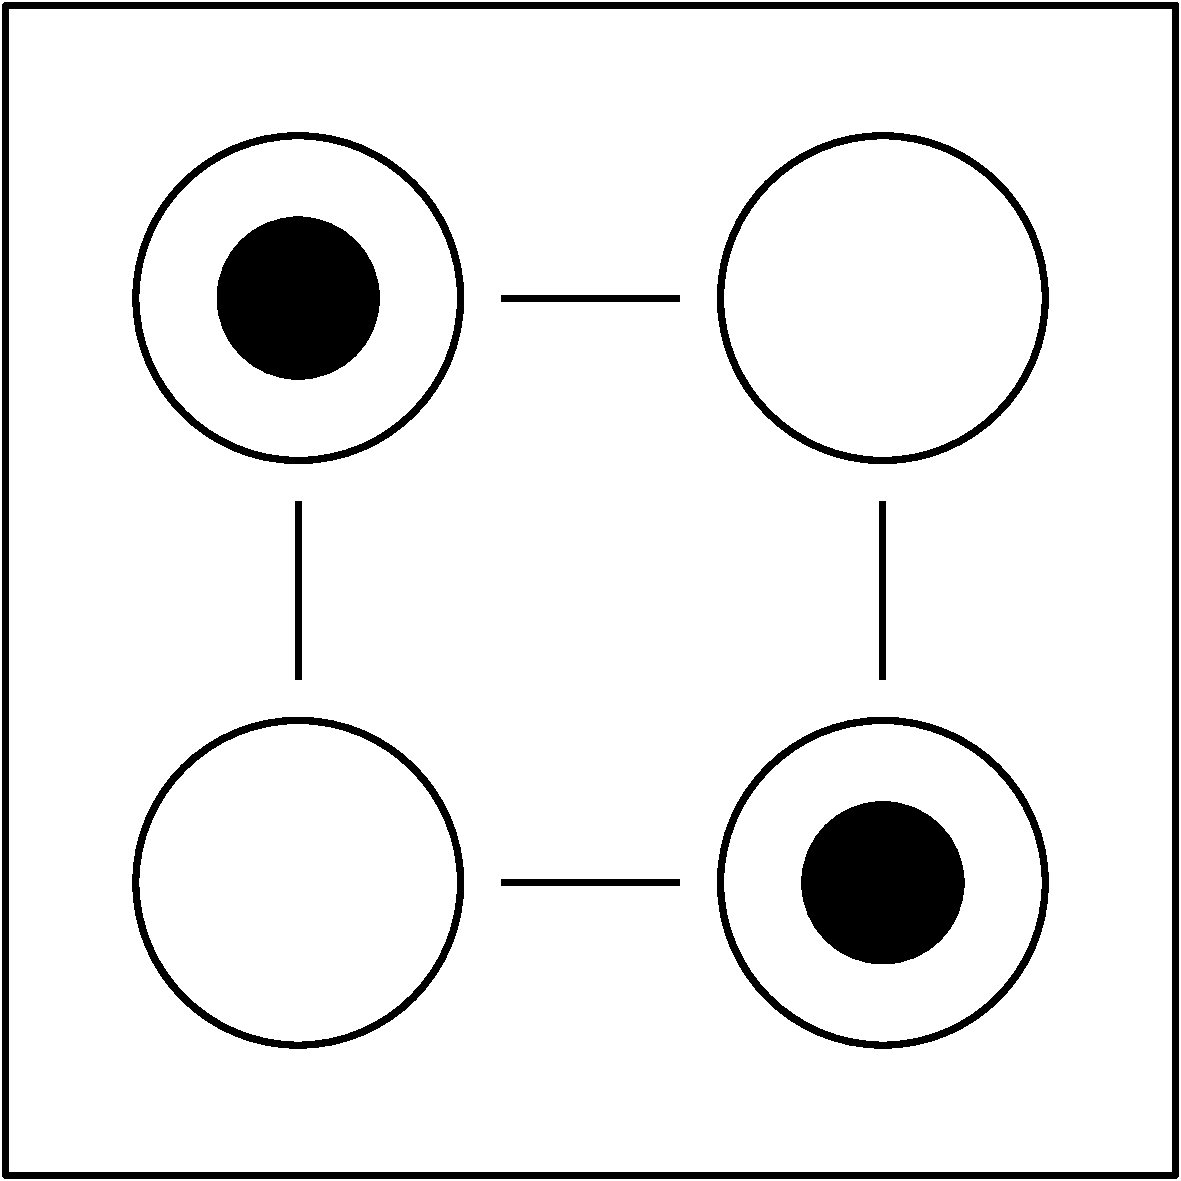
\includegraphics[width=0.35\textwidth]{../img/pregled/single_cell.pdf}
	\caption{Shema kvantne celice. Poleg štirih kvantnih pik in tunelov sta prikazana še dva elektrona, ki se nahajata v piki levo zgoraj in v piki desno spodaj.}
	\label{img-pregled-single-cell}
\end{figure}

V kvantni celici sta ujeta dva elektrona.
Vsak od njiju se lahko nahaja v eni izmed štirih kvantnih pik, med katerimi se lahko pomika prek tunelov, ki jih povezujejo.
Elektrona se zaradi odbojnih sil med njima v odsotnosti zunanjih vplivov postavita v eno izmed dveh stabilnih stanj, prikazanih na sliki \ref{img-pregled-2states}.

\begin{figure}[h]
	\centering
	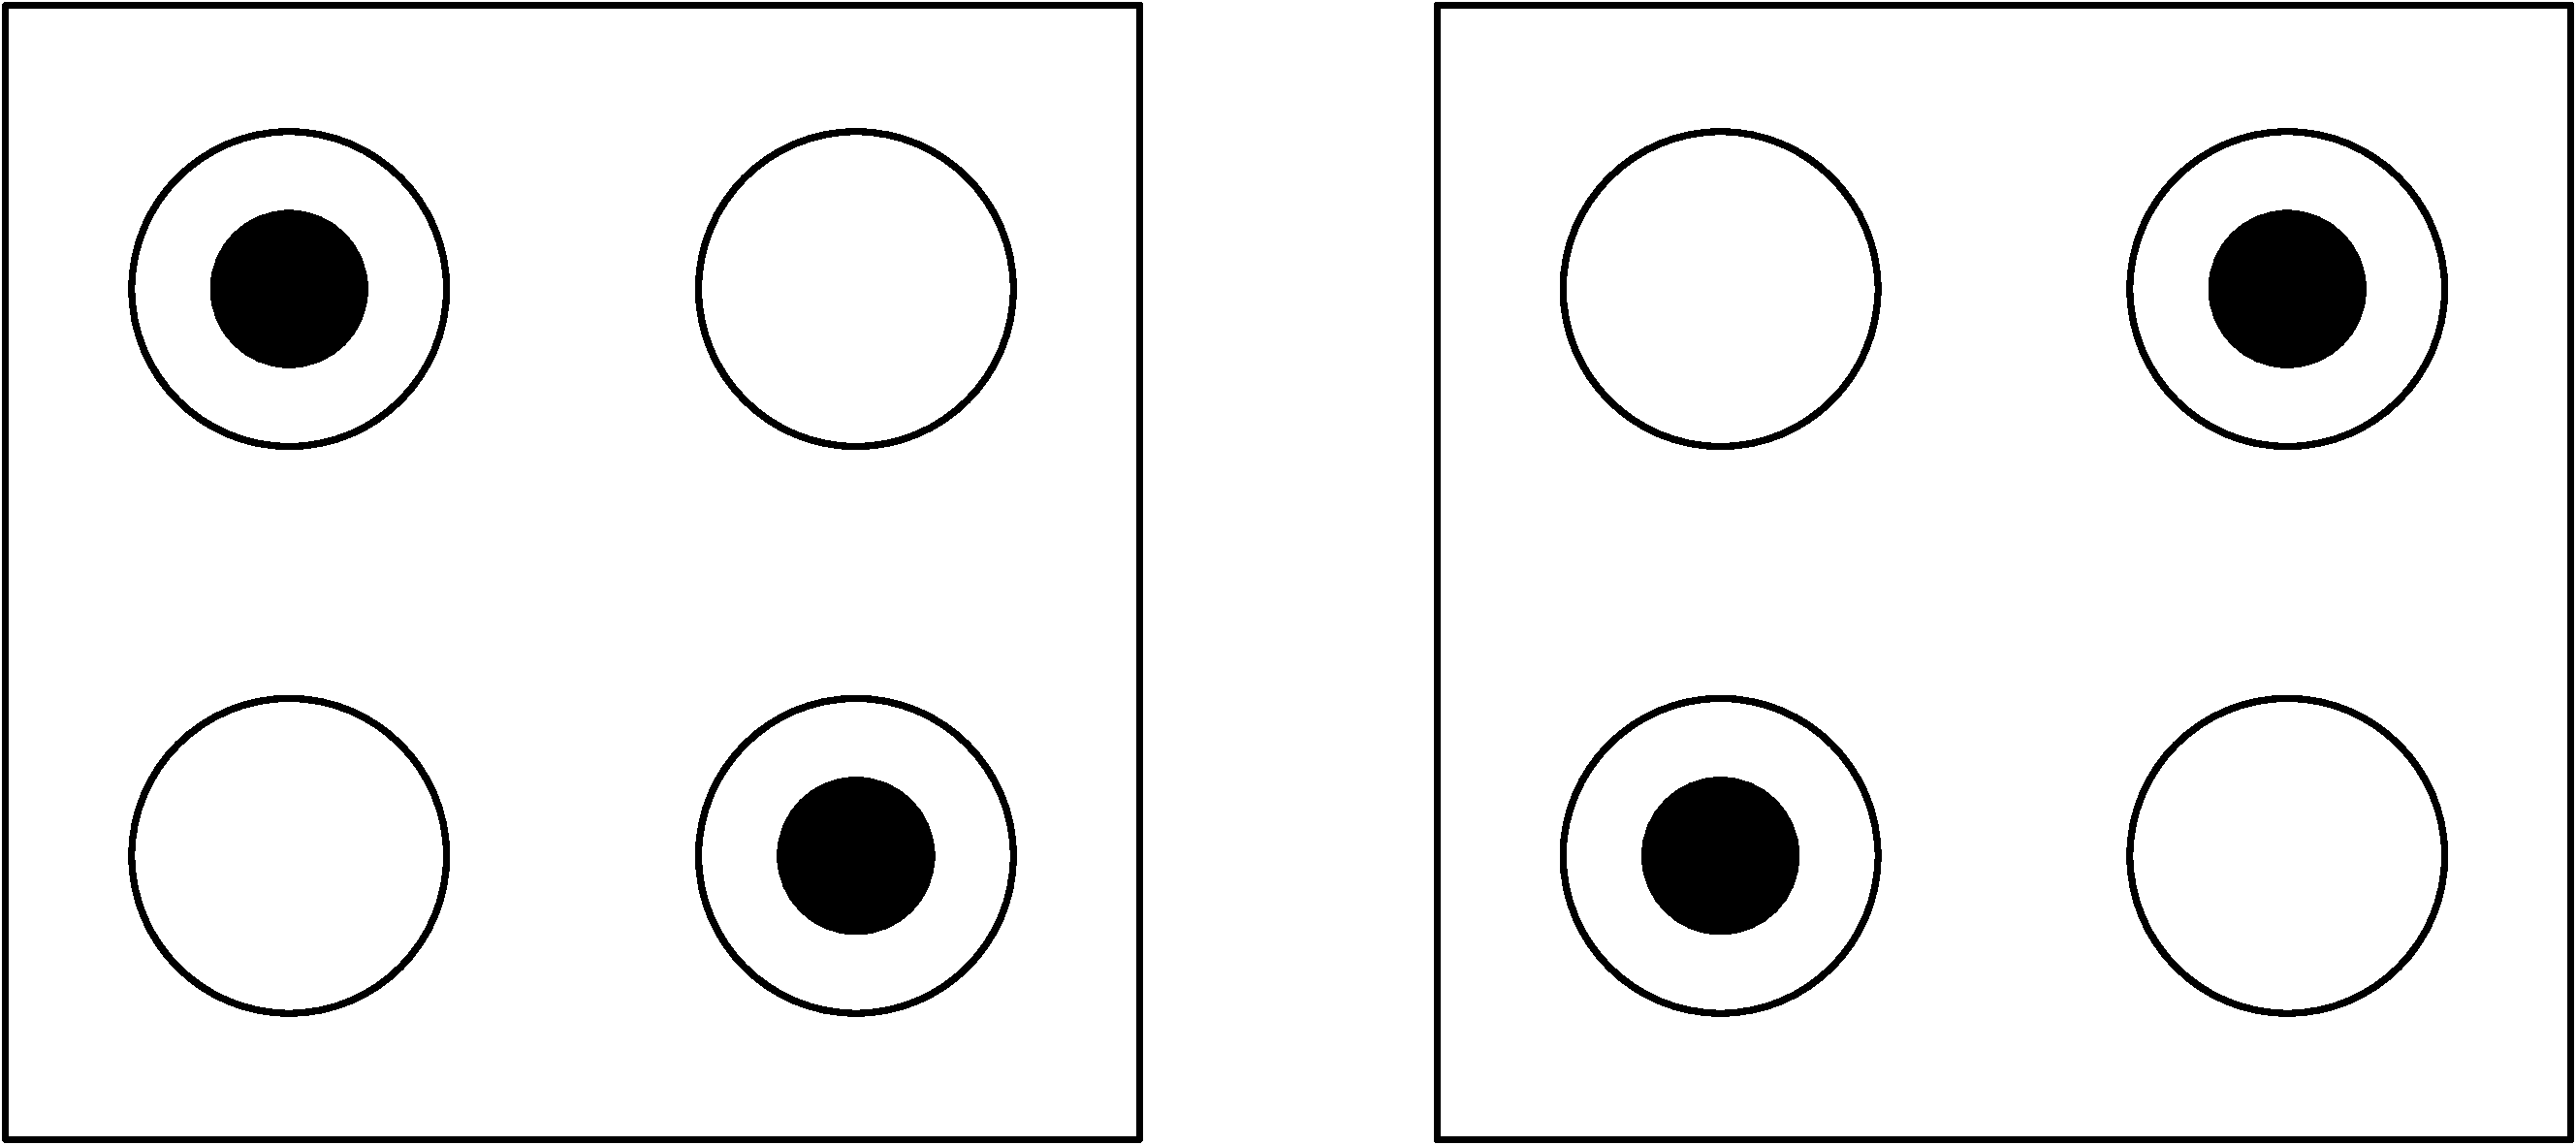
\includegraphics[width=0.65\textwidth]{../img/pregled/2states.pdf}
	\caption{Stabilni stanji kvantne celice. Na levi je prikazano stanje $P = -1$, na desni pa stanje $P = 1$.}
	\label{img-pregled-2states}
\end{figure}

Stanje $P = -1$ interpretiramo kot logično vrednost $0$, stanje $P = 1$ pa kot logično vrednost $1$ \cite{lent_1993}.
Tuneli med pikami so opremljeni s pregradami.
Elektrona lahko prosto prehajata med pikami, dokler pregrade niso vzpostavljene.
Vzpostavitev pregrad prehajanje elektronov onemogoči, kar nam omogoča, da stanje celice odčitamo.
Take celice označujemo kot izhodne.
Celico lahko tudi prisilimo, da zasede določeno stanje.
Take celice označujemo kot vhodne.

Kvantni celični avtomat je konstrukt, ki vsebuje eno ali več kvantnih celic, ki zaradi medsebojne bližine interaktirajo druga z drugo.
Sile med elektroni težijo k vzpostavitvi stanja z najmanjšo skupno energijo.
V odsotnosti zunanjih sil se kvantna celica postavi v eno izmed dveh stabilnih stanj z verjetnostjo $\frac{1}{2}$, ampak če so v njeni bližini druge kvantne celice, se ta verjetnost spremeni.
S pravilno postavitvijo celic lahko dosežemo, da se avtomat obnaša kot tradicionalna Boolova preklopna funkcija.

Gradnjo kompleksnejših struktur pričnemo z osnovnimi gradniki.
Osnovni gradniki predstavljajo poln funkcijski nabor, s katerim lahko implementiramo poljubno preklopno funkcijo.
Najenostavnejši gradnik je vodilo, prikazano na sliki \todo.

\todo: slika vodila

Vodila preslikajo vhodno vrednost na izhod.
Uporabljamo jih za povezovanje gradnikov v avtomatu.
Drugi gradnik je negator, prikazan na sliki \todo.

\todo: slika negatorja

Negatorje lahko uporabimo tudi kot diagonalno vodilo, kjer je dolžina takega vodila sodo število.
Primer take uporabe je prikaza na sliki \todo.

\todo: slika vodila iz negatorjev

Zadnji osnovni gradnik so večinska oz.~majoritetna vrata, prikazana na sliki \todo.

\todo: slika majoritetnih vrat

Izhod majoritetnih vrat zavzame večinsko vrednost na treh vhodih.
Z vezavo konstante na enega izmed vhodov majoritetnih vrat dobimo gradnik, ki predstavlja konjunkcijo ali disjunkcijo, kot je prikazano na sliki \todo.

\todo: tabela AND, OR iz majoritetnih

Tok podatkov v avtomatu usmerjamo s pomočjo urinih con.
Vsaki celici dodelimo eno izmed štirih urinih con, ki se ciklično izmenjujejo.
Tako omogočimo logično separacijo delov avtomata in način interakcije med njimi.
Primer avtomata z ločenimi urinimi conami je prikazan na sliki \todo.

\todo: slika avtomata z različnimi urinimi conami

\subsection{Problematika pomnenja}

Ko je ura odsotna, je stanje kvantne celice v odsotnosti zunanjih sil nedeterministično.
Tako kvantnih celic samih ne moremo uporabiti za hrambo podatkov.
Uvedba ure omogoča, da kvantne celice spravimo v zaklenjeno stanje, v katerem prehajanje elektronov med pikami ni mogoče, kar pomeni, da je stanje zaklenjene kvantne celice deterministično.
Za pomnenje potrebujemo še način za nadzor stanja, ki naj ga zaklenjena celica zavzame.
To lahko dosežemo z veriženjem celic, ki ne pripadajo isti urini coni.
Takšna veriga je prikazana na sliki \todo.

\todo: slika verige s sekvenčnimi urinimi conami

Za samostojno pomnenje to verigo sklenemo v obroč, prikazan na sliki \todo.

\todo: slika obroča s sekvenčnimi urinimi conami

V obroču se stanje med potekom urinega cikla ohranja, kot je prikazano na sliki \todo.

\todo: shema / tabela s stanji v obroču med urinim ciklom (simulacija v QCA Designer)

Za smiselno uporabo želimo to strukturo prirediti tako, da lahko hranjeno stanje poljubno nastavljamo.
Kako to storimo, je stvar implementacije.
V nadaljevanju bomo predstavili nekaj obstoječih implementacij pomnilnih struktur.

\subsection{Reverzibilno procesiranje (?)}



\section{Pomnilne celice}
Za gradnjo sekvenčnih vezij poleg logičnih vrat potrebujemo tudi pomnilne celice. Osnovne pomnilne celice, ki omogočajo hranjenje enega bita informacije, so RS (Reset Set), JK (Jump Kill), T (Trigger) in D (Delay) pomnilna celica. 


\subsection{Obstoječe implementacije}
V članku \cite{quantum_dot} iz leta 2003 so predstavljene implementacije štirih osnovnih pomnilnih celic. Vse celice porabijo en urin cikel za procesiranje vhodov. Pri postavitvi celic vir uporablja pravilo čimbolj preprostih oblik urinih con in čimmanj le-teh. Po drugi strani pa so nekatere celice zasukane za kot $ 45^{\circ} $ ali zamaknjene za polovico svoje velikosti, kar lahko negativno vpliva na izvedljivost implementacije. Vir uporablja križanje linij, kar je možno doseči z uporabo alternirajočega vodila (rotiranih celic). \\ Drugi vir \cite{a_novel_approach} iz leta 2018 porabi manj prostora in celic ter ponudi tako izhodno stanje $Q$ kot njegovo negacijo $\bar{Q}$, so pa zato urine cone bolj kompleksne. Po drugi strani ta vir uporablja manj stabilne negatorje kot prvi.

\subsection{Reverzibilne implementacije (?)}

\subsection{Ideje in popravki (?)}


\section{Implementacija}
V tem poglavju bomo primerjali predlagane implementacije pomnilnih celic.\\
\todo: primerjaj implementacije: potratnost, izvedljivost, konsistentnost\\
\todo: vsem slikam dodati naslov in se sklicati v besedilu\\
\todo: ali štejemo kot negator tudi določene povezave, ki niso standardna negatorja (navaden in dvojni), ampak opravljajo isto funkcijo? --> vir \cite{quantum_dot}

\begin{tabular}{|c|c|c|c|c|}
\hline 
Pomnilna celica & Vir & Število majoritetnih vrat & Število negatorjev & Število celic \\ 
\hline 
\multirow{2}{*}{D} & \cite{quantum_dot} & 3 & 2 & 68 \\ 
& \cite{a_novel_approach} & 4 & 2 & 43 \\ 
\hline 
\multirow{2}{*}{JK} & \cite{quantum_dot} & 5 & 2 & 90 \\ 
& \cite{a_novel_approach} & 6 & 2 & 78 \\ 
\hline 
\multirow{2}{*}{RS} & \cite{quantum_dot} & 4 & 1 & 76 \\ 
& \cite{a_novel_approach} & 4 & 2 & 38 \\ 
\hline 
\multirow{2}{*}{T} & \cite{quantum_dot} & 5 & 4 & 92 \\  
& \cite{a_novel_approach} & 6 & 2 & 81 \\ 
\hline 
\end{tabular} 

\subsection{D pomnilna celica}
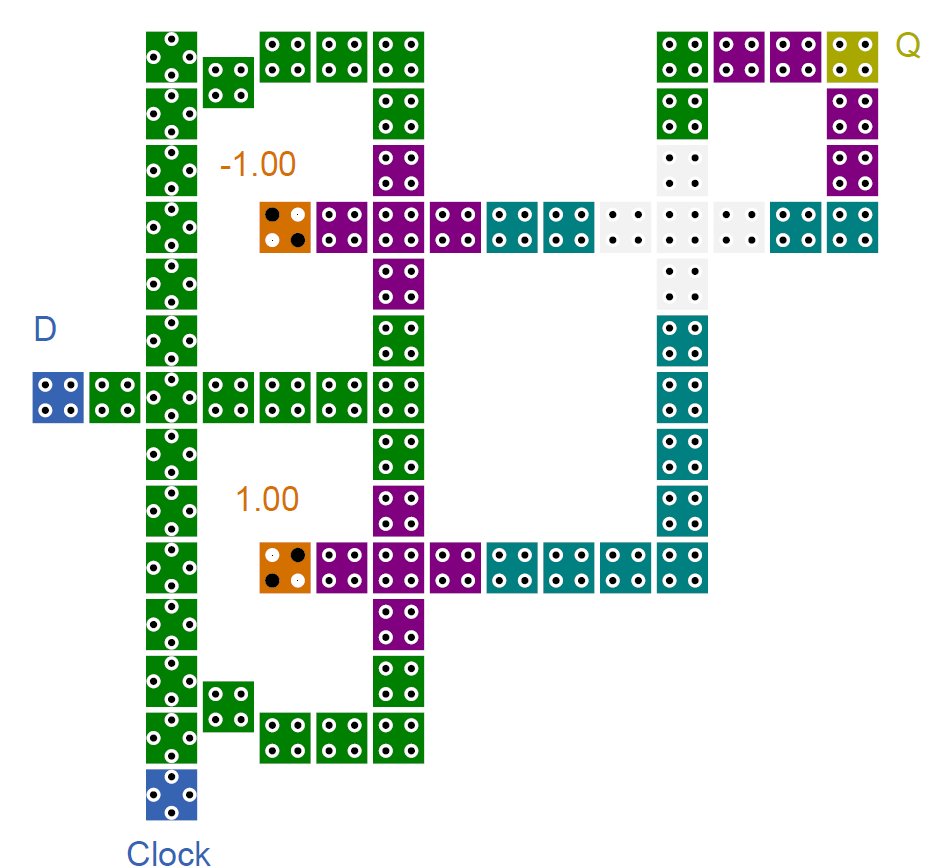
\includegraphics[scale=0.4]{../img/vir_4/d.png} 
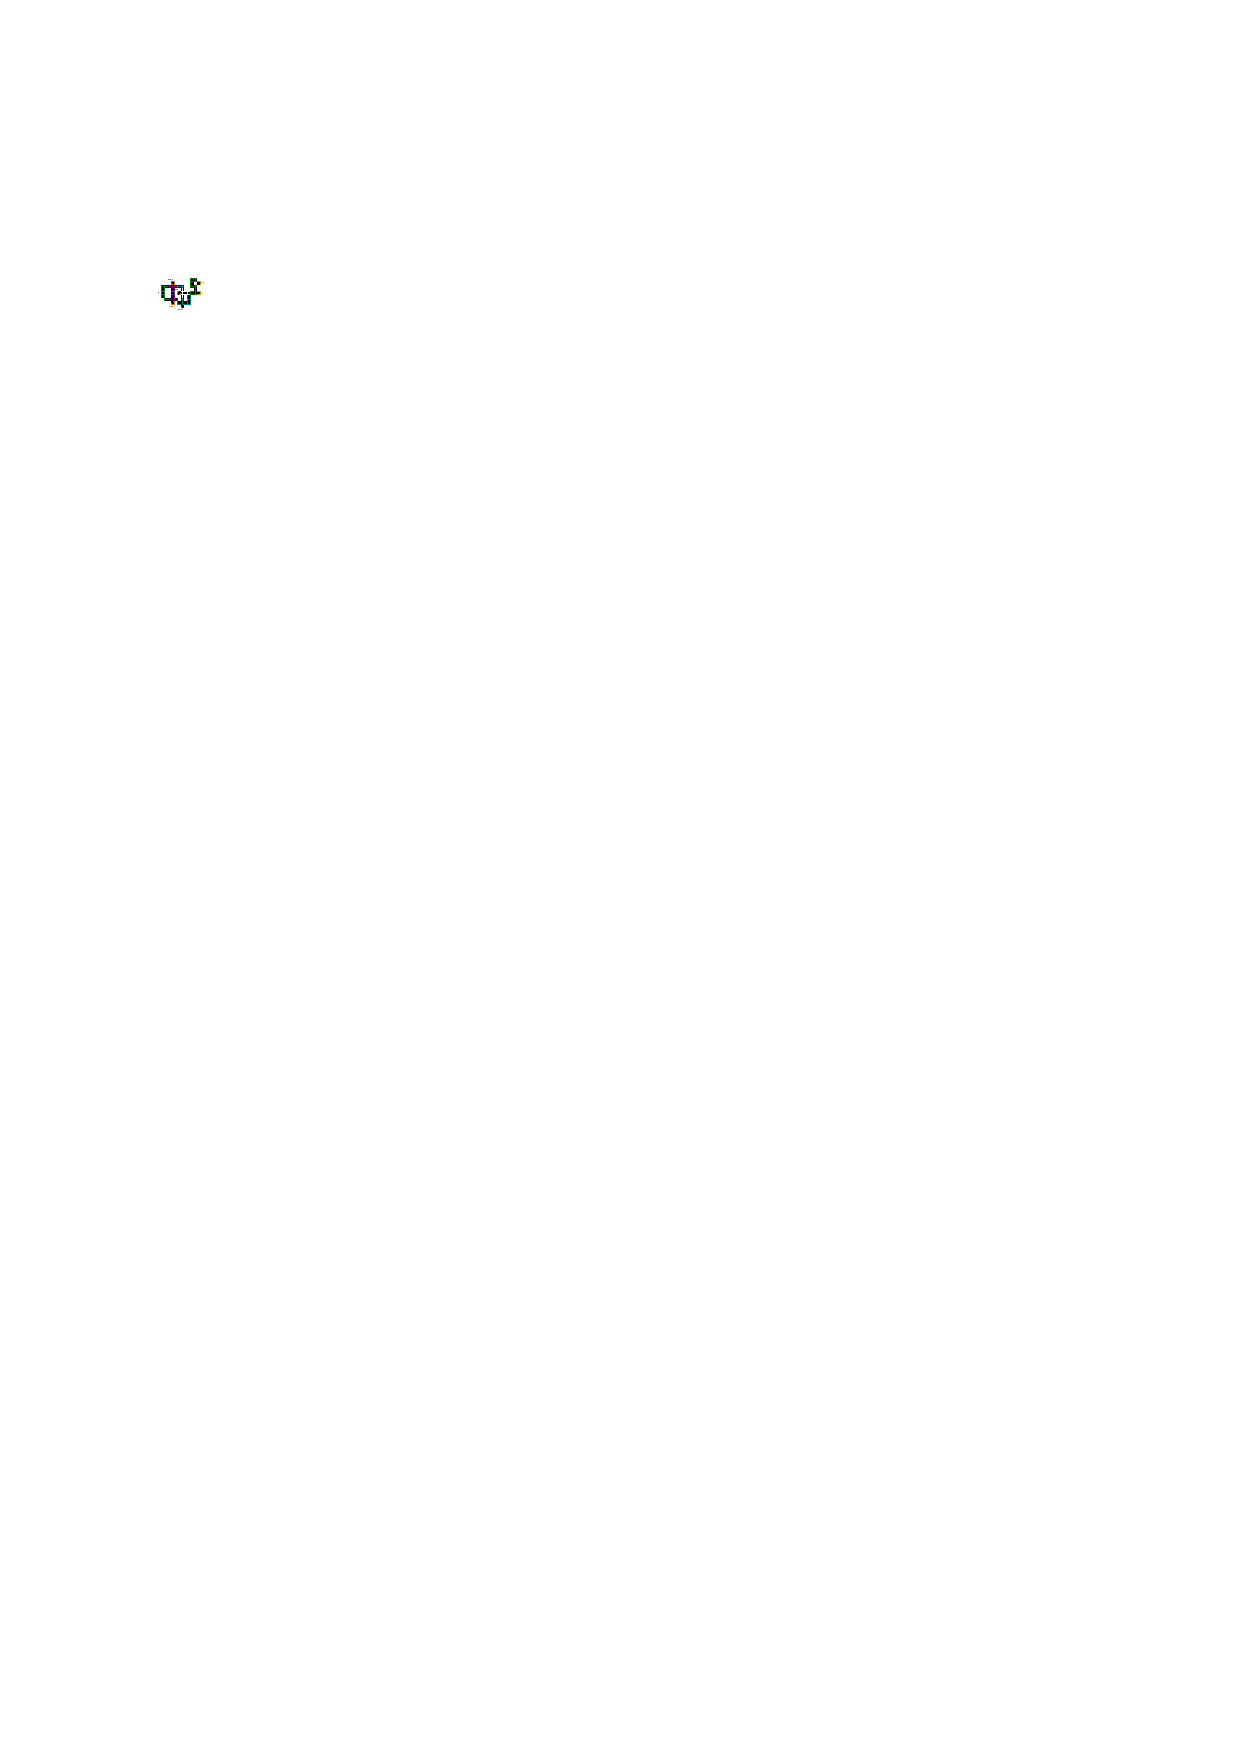
\includegraphics[scale=0.32]{../img/vir_5/d.png} 

\subsection{JK pomnilna celica}
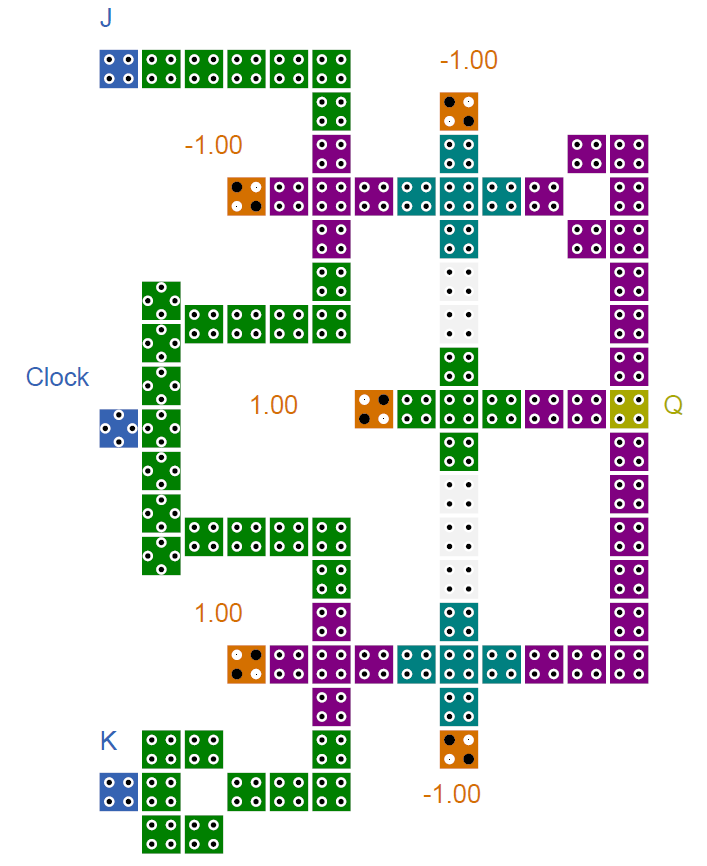
\includegraphics[scale=0.5]{../img/vir_4/jk.png} 
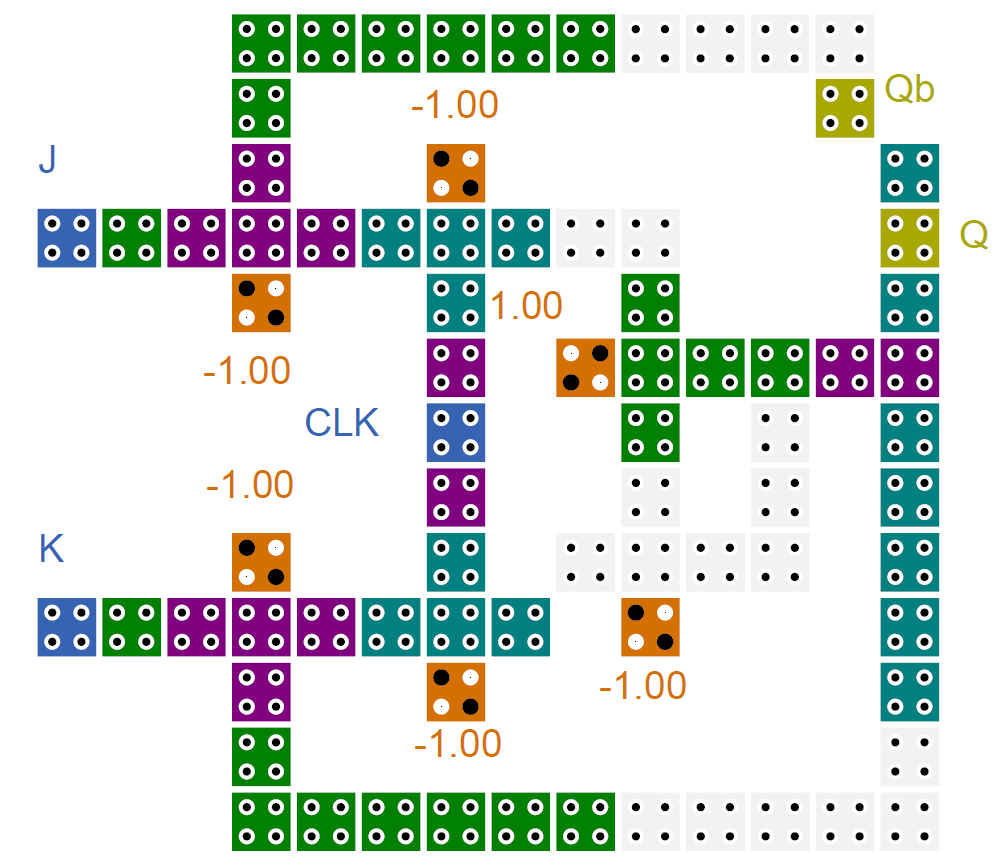
\includegraphics[scale=0.35]{../img/vir_5/jk.png} 

\subsection{RS pomnilna celica}
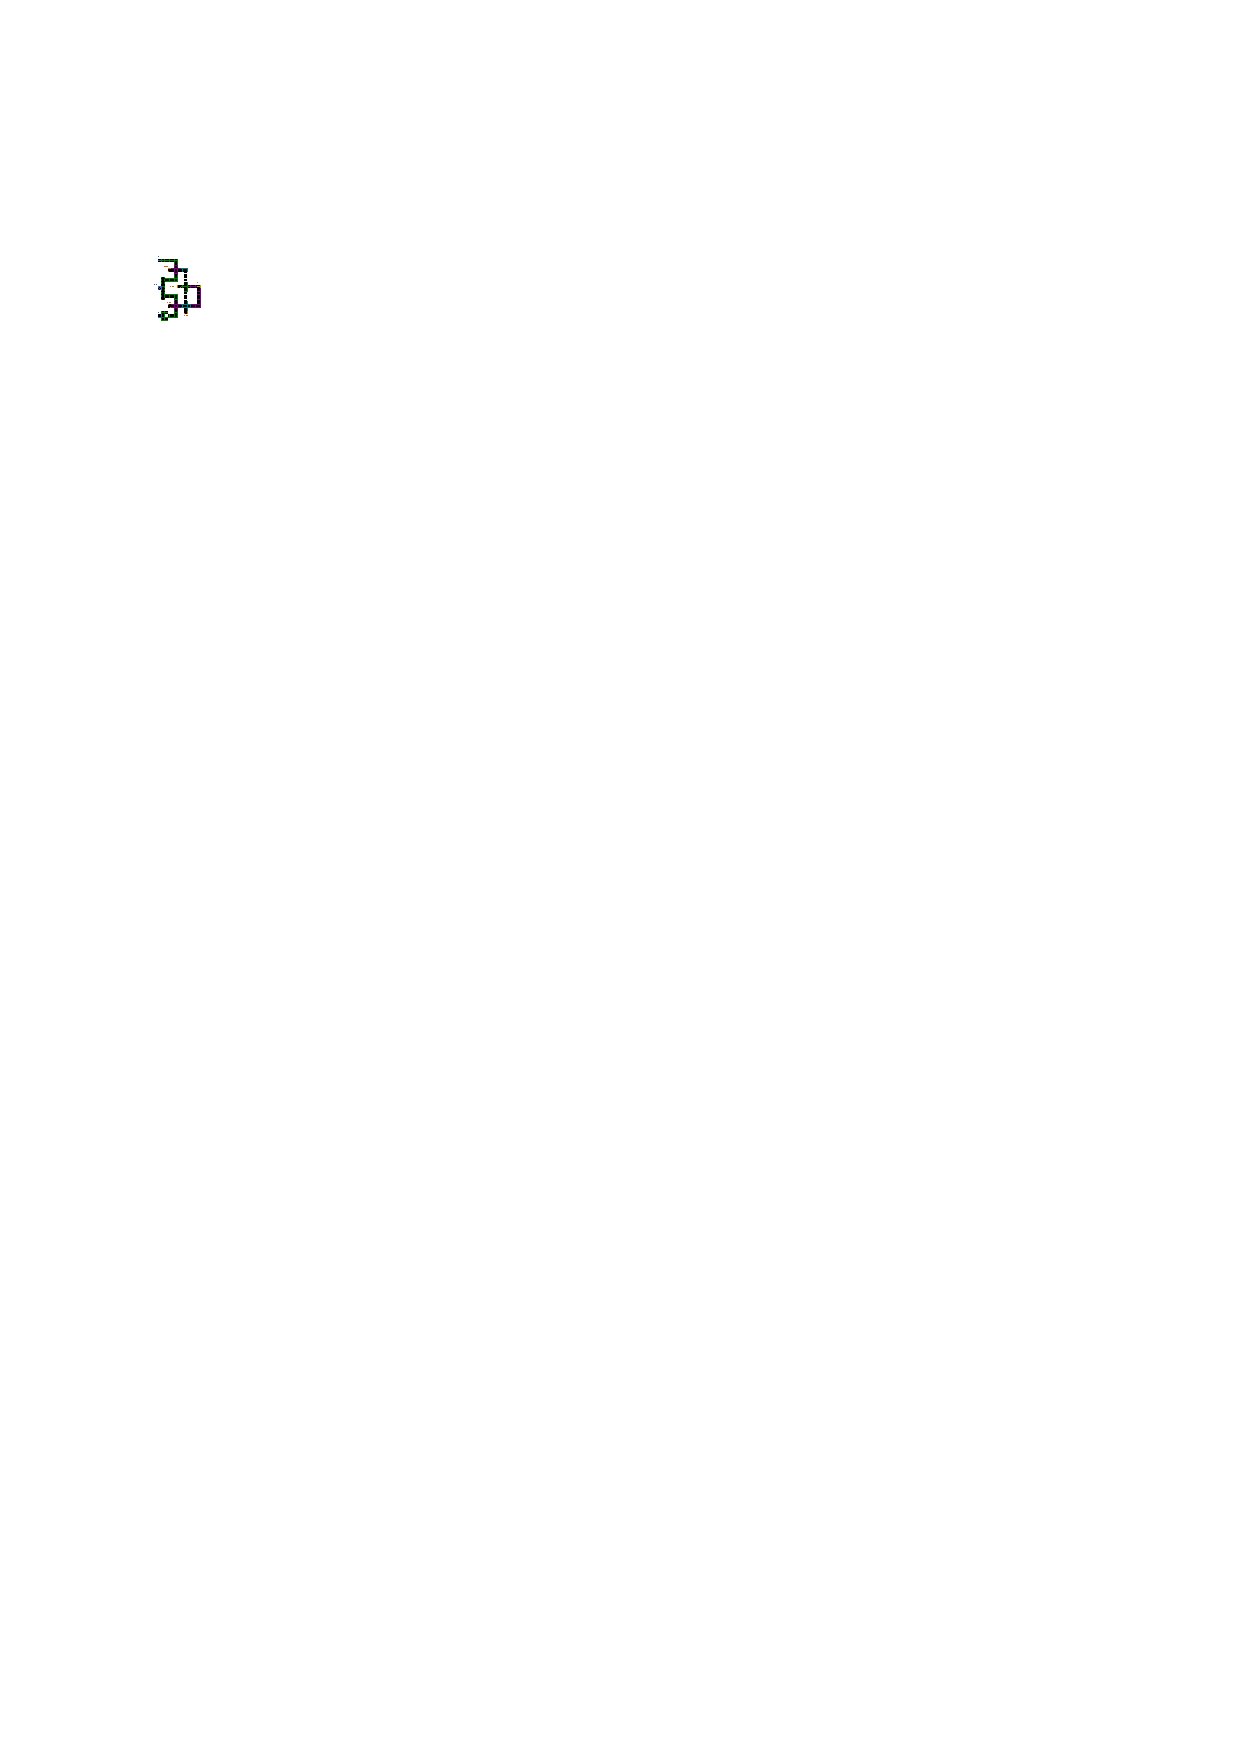
\includegraphics[scale=0.5]{../img/vir_4/sr.png} 
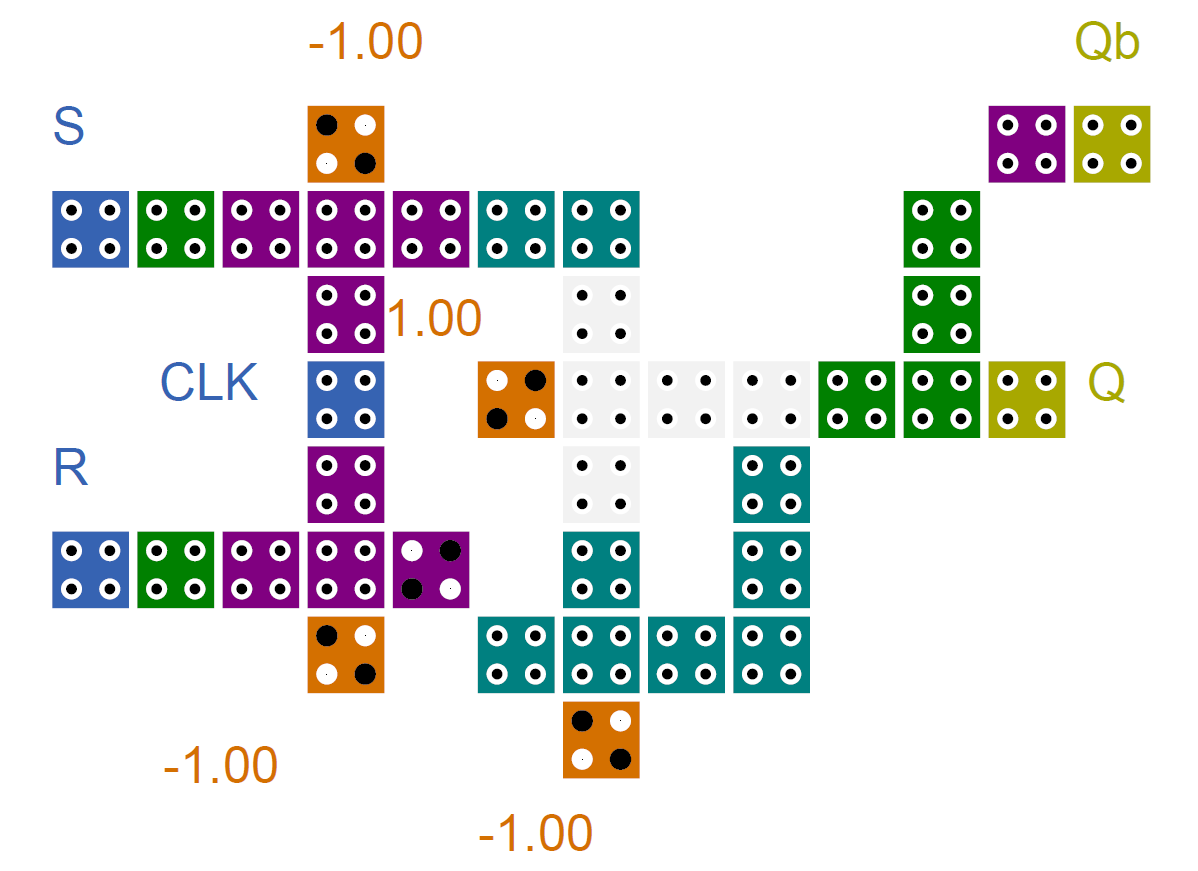
\includegraphics[scale=0.3]{../img/vir_5/rs.png} 

\subsection{T pomnilna celica}
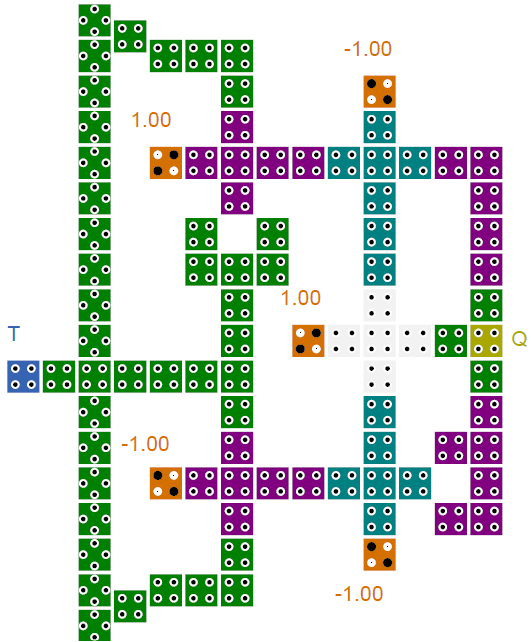
\includegraphics[scale=0.6]{../img/vir_4/t.png} 
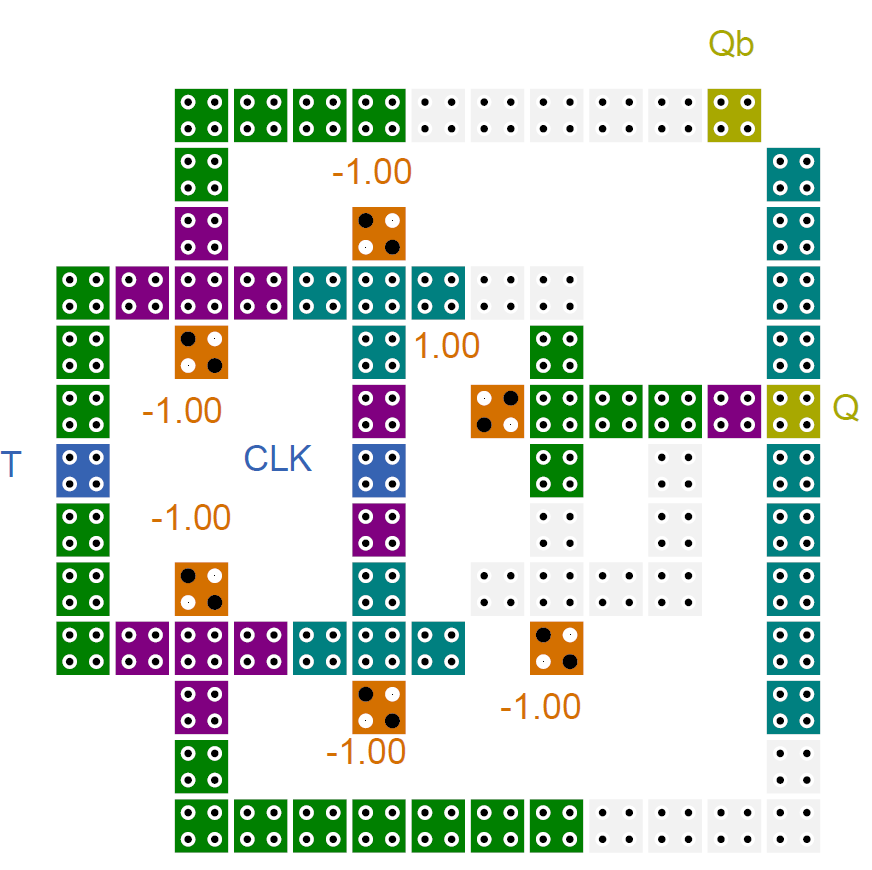
\includegraphics[scale=0.4]{../img/vir_5/t.png} 


\subsection{Analiza delovanja}
\subsubsection{D pomnilna celica}
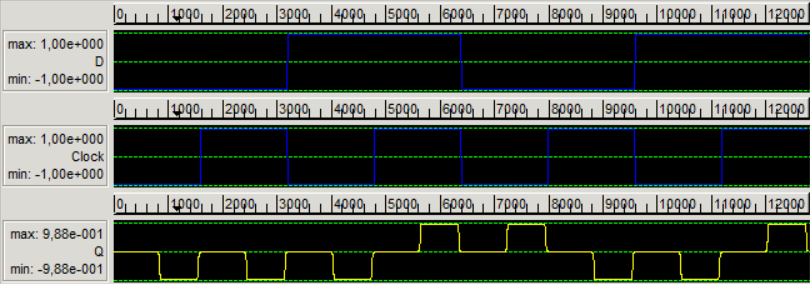
\includegraphics[scale=0.5]{../img/vir_4/sim_d.png} \\
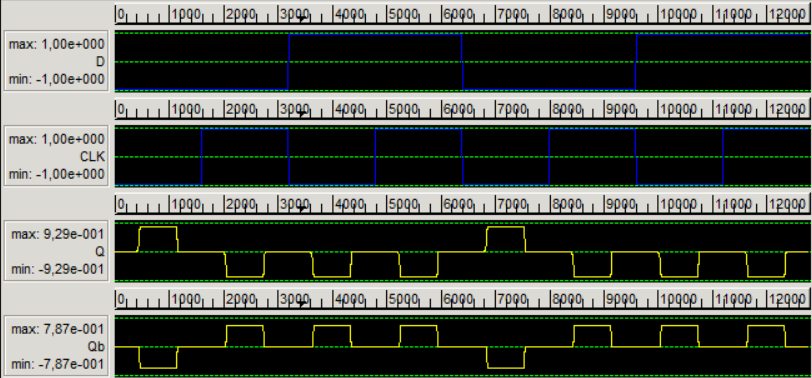
\includegraphics[scale=0.5]{../img/vir_5/sim_d.png}

\subsubsection{JK pomnilna celica}
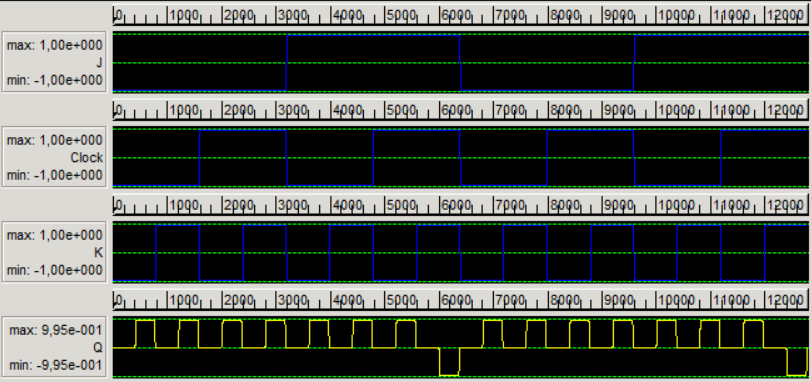
\includegraphics[scale=0.5]{../img/vir_4/sim_jk.png} \\
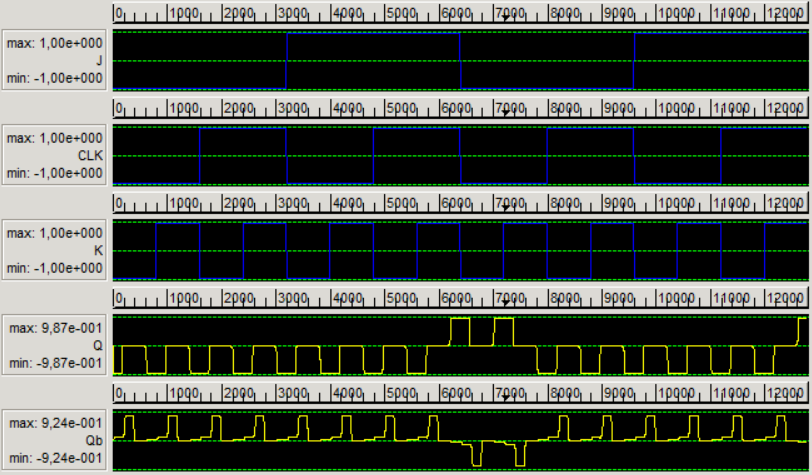
\includegraphics[scale=0.5]{../img/vir_5/sim_jk.png}

\subsubsection{RS pomnilna celica}
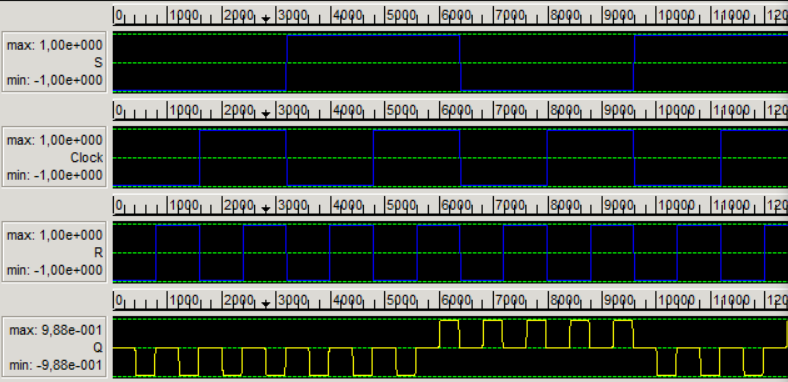
\includegraphics[scale=0.5]{../img/vir_4/sim_sr.png} \\
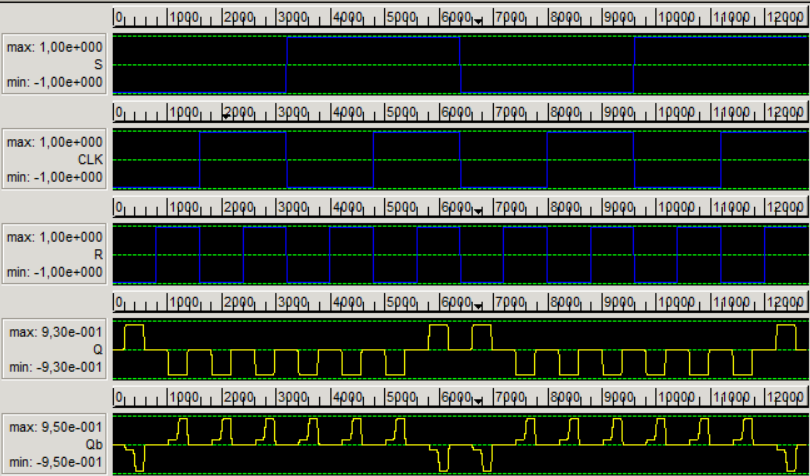
\includegraphics[scale=0.5]{../img/vir_5/sim_rs.png}

\subsubsection{T pomnilna celica}
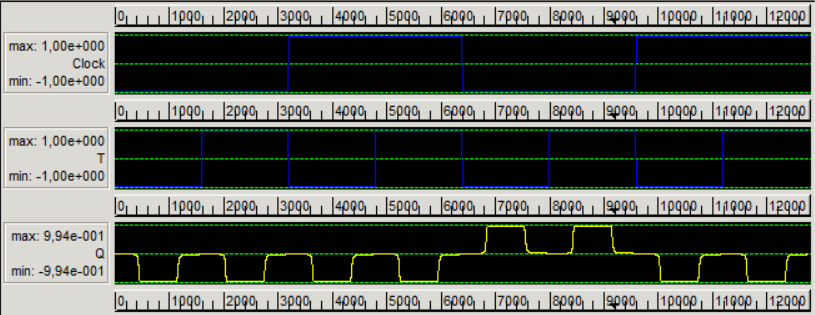
\includegraphics[scale=0.5]{../img/vir_4/sim_t.png} \\
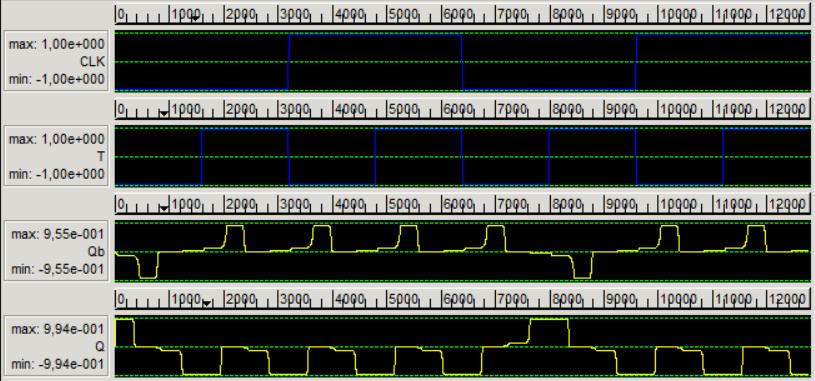
\includegraphics[scale=0.5]{../img/vir_5/sim_t.png} 

\section{Zaključek}
\todo: kratek povzetek glavnih ugotovitev + smernice za nadaljnje delo

\bibliographystyle{babplain}
\bibliography{pomnjenje} 

\end{document}
